\documentclass[serif,mathserif]{beamer}
\usepackage{amsmath, amsfonts, epsfig, xspace}
\usepackage{algorithm,algorithmic}
\usepackage{pstricks,pst-node}
\usepackage{multimedia}
\usepackage[normal,tight,center]{subfigure}
\setlength{\subfigcapskip}{-.5em}
\usepackage{beamerthemesplit}
\usetheme{lankton-keynote}

\author[Ingo Fischer]{Ingo Fischer}

\title[Messaging\hspace{2em}\insertframenumber/\inserttotalframenumber]{Messaging}

\date{} %leave out for today's date to be insterted

\institute{ACME Company}

\begin{document}

\maketitle

% \section{Introduction}  % add these to see outline in slides

\begin{frame}
\frametitle{Main Concepts}
Besides choosing a Message Protocol and the corresponding Messaging Architecture, 
we should define some main concepts that are independent of the Messaging solution we choose.
\end{frame}

\begin{frame}
\frametitle{Main Concepts}
\begin{itemize}
  \item Completely abstract underlying transport mechanism
  \begin{itemize}
    \item separate transport logic
    \item configure transport with configuration files
    \item Service lookup (how?)
    \item later: allow dynamic change of transport without
    restarting/reconfiguring services (how?)
  \end{itemize}
\end{itemize}
\end{frame}

\begin{frame}
\frametitle{Zookeeper}
\begin{figure}[t]
\centering
\subfigure[Overview]{
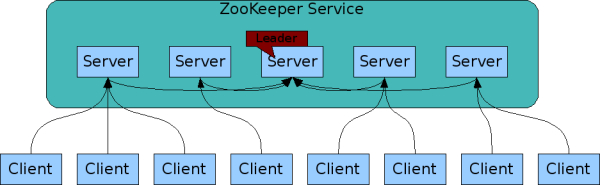
\includegraphics[width=10cm]{images/zkservice}}
\end{figure}
\end{frame}

\begin{frame}
\frametitle{Questions}
\end{frame}
\end{document}